% WWW'27 submission — Progress-Aware Bisimulation Heads (draft v2.0, 2026-10-07)
% Compile: pdflatex main && bibtex main && pdflatex main x2
\documentclass[sigconf]{acmart}

%% ---------- WWW27 boilerplate (replace at camera-ready) ----------
\setcopyright{none}
\settopmatter{printacmref=false}
\acmConference[WWW'27]{The Web Conference}{April 2027}{TBD}
\acmYear{2027}
\acmDOI{}
\acmISBN{}
\acmPrice{}
%% ------------------------------------------------------------

\usepackage{booktabs}
\usepackage{multirow}
\usepackage{subcaption}
\usepackage{graphicx}
\usepackage{amsmath}
% amssymb omitted: conflicts with acmart newtxmath (Bbbk already defined)
\usepackage{algorithm}
\usepackage{algpseudocode}
\usepackage{xcolor}
\newcommand{\method}{PABH}
\newcommand{\todo}[1]{\textcolor{red}{[TODO: #1]}}
\newcommand{\gtext}{\ensuremath{g_{\text{text}}}}
\newcommand{\gset}{\ensuremath{g_{\text{set}}}}

\begin{document}

\title{Progress-Aware Bisimulation Heads for Step-Level Credit\\Assignment in LLM Agents}

%% ---------- authors (placeholder) ----------
\author{Anonymous Author(s)}
\affiliation{\institution{Anonymous Institution}\country{}}
\email{anon@example.com}

%% ---------- abstract ----------
\begin{abstract}
Group-based reinforcement learning methods such as GiGPO assign step-level
credit by comparing actions that share an identical \emph{anchor state}.
BiPACE relaxes exact matching with behavioral clustering over the actor's
hidden states, but the resulting distance metric is purely syntactic: it
inherits whatever state information leaks into the hidden representation,
conflating states at different stages of task progress.
We propose a \emph{progress-aware bisimulation head}---a lightweight,
frozen-backbone linear projection trained online with a MICo-style metric
loss whose reward anchor is derived from \emph{task progress} rather than
terminal outcomes. The method is a three-layer stack: (i) structured
progress sets $\gset$ injected into the anchor observation;
(ii) a trained value-equivalence metric with interchangeable rule-based
process-reward (PRM) or progress-set Jaccard anchors;
(iii) purity-preserving consumption of the metric in cluster-based
advantage estimation.
Across three interactive environments with Qwen2.5-1.5B/7B-Instruct, our
method improves peak success over strong BiPACE-Q reproductions by
+4.6--5.4\,pp (ALFWorld 1.5B, 5 seeds, 95.2$\pm$1.4\%), +1.4/+1.7\,pp
(WebShop 1.5B/7B), and +2.9\,pp (ScienceWorld 1.5B, 3 seeds, 89.6\%),
with all three seeds dominating every baseline seed on ScienceWorld.
A controlled decomposition shows the trained metric---not the textual
state redefinition---carries the 1.5B gain (+5.3\,pp vs.\ $-$0.4\,pp),
while both layers contribute modestly at 7B, explaining the
scale-dependence of representation quality.
A 16-run retrospective purity analysis further shows that group
contamination (same-observation/different-progress states) doubles over
training and correlates with final success at $r=-0.75$ at 7B, while the
community's coverage metric (singleton rate) is uncorrelated
($r=+0.02$)---evidence that \emph{purity, not coverage, is the right
optimization target}.
\end{abstract}

\begin{CCSXML}
<ccs2012>
<concept><concept_id>10010147.10010257.10010258.10010261</concept_id>
<concept_desc>Computing methodologies~Reinforcement learning</concept_desc>
<concept_significance>500</concept_significance></concept>
<concept><concept_id>10010147.10010178.10010199.10010202</concept_id>
<concept_desc>Computing methodologies~Multi-agent systems</concept_desc>
<concept_significance>300</concept_significance></concept>
</ccs2012>
\end{CCSXML}
\ccsdesc[500]{Computing methodologies~Reinforcement learning}
\ccsdesc[300]{Computing methodologies~Multi-agent systems}

\keywords{LLM agents, reinforcement learning, credit assignment,
bisimulation metrics, group-based policy optimization}

\maketitle

%% ======================================================================
\section{Introduction}
\label{sec:intro}

Training large language model (LLM) agents with reinforcement learning
(RL) has converged on \emph{group-based} estimators (RLOO, GRPO) that
replace learned critics with within-group relative advantages. For
multi-step agent tasks---web shopping, household control, science
experiments---GiGPO~\cite{gigpo} extends the idea to the step level:
actions are compared only against other actions taken at the
\emph{same} environment state, discovered retroactively by hashing
repeated observations across trajectories. The episode-level group
baseline thus becomes a \emph{state}-level one, sharpening credit
assignment at negligible cost.

Exact state hashing, however, is brittle in text environments:
behaviorally equivalent states rarely produce byte-identical
observations. BiPACE~\cite{bipace} relaxes the match with behavioral
clustering over the actor's hidden states (BiGPO) and re-centers
advantages on same-action peers (PACE). The step-level group becomes
\emph{approximate}---a learned equivalence relation---and the quality of
credit assignment now hinges entirely on the \textbf{distance metric
over states}.

We identify two previously unaddressed failure modes of hidden-state
cosine distance as a bisimulation proxy:

\begin{enumerate}
\item \textbf{Progress blindness.} The anchor observation in agent
pipelines typically contains only single-step action feedback
(e.g., ``You pick up the pillow''). Two states at very different stages
of task completion can be near-identical in this representation, so the
cluster mixes trajectories with different remaining values---a temporal
confound that directly contaminates the group baseline
(\S\ref{sec:e2}: 18--31\% of exact-observation clusters are
progress-inconsistent, and the contamination \emph{doubles} over
training).
\item \textbf{Untrained metric.} The hidden representation is optimized
for token prediction, not value equivalence. Nothing in the training
loop encourages $\|z(s)-z(s')\|$ to reflect the \emph{decision-relevant}
similarity of $s$ and $s'$.
\end{enumerate}

We address both with a \textbf{progress-aware bisimulation head}
(\method): a single linear projection over a frozen LLM layer, trained
online with a MICo-style bisimulation loss~\cite{micobisim} whose reward
anchor is grounded in \emph{task progress}---either a rule-based process
reward or a Jaccard distance over completed-subgoal sets. The head is
trained on the same rollouts that feed the PPO update (0.39M parameters,
$<$2\% step time), and its output replaces raw hidden states in BiGPO
clustering.

Our contributions:

\begin{itemize}
\item \textbf{Method.} A three-layer stack for step-level grouping in
group-based agent RL: progress-set state redefinition $(g,o)$, a
progress-grounded trained metric, and purity-preserving consumption.
Two interchangeable metric anchors (event PRM; progress-set Jaccard)
make the anchor granularity an explicit, ablatable design choice
(\S\ref{sec:method}).
\item \textbf{Results across three environments.} Consistent gains over
same-pipeline BiPACE-Q reproductions: ALFWorld 1.5B 95.2$\pm$1.4\%
(5 seeds, +4.6--5.4\,pp; official BiPACE-Q 93.5$\pm$1.2), ALFWorld 7B
95.3 ($\times$2 seeds), WebShop +1.4/+1.7\,pp (1.5B/7B), ScienceWorld
1.5B 89.6\% (3 seeds, all dominating baseline, +2.9\,pp) and 7B
final +3.2\,pp (\S\ref{sec:main}).
\item \textbf{Attribution.} A mid-arm ablation decomposes the 1.5B gain:
progress-set text injection alone contributes $\approx$0, while the
trained head contributes +5.3\,pp; at 7B the two layers split
+1.2/+0.8\,pp---a scale-dependent account of when metric learning pays
(\S\ref{sec:attrib}).
\item \textbf{Purity over coverage.} A zero-GPU retrospective analysis
of 16 runs shows group contamination rises through training and
predicts final success ($r=-0.75$ at 7B), while singleton rate is
uninformative ($r=+0.02$)---overturning the field's default
``lower singleton is better'' heuristic (\S\ref{sec:e2}).
\end{itemize}

%% ======================================================================
\section{Background}
\label{sec:background}

\paragraph{Group-based step-level credit.}
GiGPO computes advantages as $A = A_{\text{episode}} + \omega
A_{\text{step}}$, where $A_{\text{episode}}$ is GRPO-style trajectory
normalization within a prompt group, and $A_{\text{step}}$ normalizes
each step's discounted return within its \emph{anchor group}---the set
of steps sharing an identical observation.

\paragraph{BiPACE.}
BiPACE replaces exact anchor matching with behavioral clustering:
anchor observations are embedded (actor hidden states at a fixed late
layer, L2-normalized) and greedily clustered by cosine distance
$\le\varepsilon$. Within each cluster, the PACE estimator partitions by
action identity and computes $A=\hat{Q}(s,a)-\hat{V}(s)$ from
same-action vs.\ all-action peer means. The cluster structure is
therefore a \emph{learned equivalence relation}---but one never trained
against any notion of value equivalence.

\paragraph{Bisimulation metrics.}
Bisimulation metrics~\cite{ferns2011bisimulation} define state distance
recursively: $d(s,s') = |r(s)-r(s')| + \gamma\,\max$ over successor-pair
distances. MICo's practical form~\cite{micobisim} fits a representation
so that $\|z(s)-z(s')\| \approx |r-r'| + \gamma\|z(s^+)-z(s'^+)\|$,
solvable with a slowly updated target network. We adopt this loss with
two modifications: the reward anchor is a \emph{dense progress signal}
rather than sparse extrinsic reward, and the head is trained on-policy
from the same rollouts that feed the PPO update.

%% ======================================================================
\section{Method}
\label{sec:method}

\subsection{Progress sets: redefining ``same state''}
\label{sec:gspec}

Let $g(s)$ be the set of subgoals completed by the time state $s$ is
reached. We instantiate $g$ per environment with rule-based parsers:

\paragraph{ALFWorld (household tasks).} Feedback is generated from a
closed set of six event templates (``You pick up the \{obj\} from the
\{rec\}'', ``You heat the \{obj\} using the \{rec\}'', \dots). We parse
each step's feedback with anchored regexes and accumulate
$(\text{predicate},\text{object})$ events; navigation and
container-opening events are deliberately excluded so that states
differing only in agent location remain bisimilar. A 6-type $\times$
3-episode walkthrough-replay validation confirmed 100\% parse coverage.

\paragraph{ScienceWorld.} We exploit the environment's dense official
task score ($0$--$100$): progress increments
$\max(\Delta\text{score},0)/100$ define a continuous process reward
(\S\ref{sec:prm}); a template parser for subgoal events is future work.

The progress set feeds three consumers: (i) as text $\gtext$ prepended
to the anchor observation, so the policy-induced embedding also sees
progress; (ii) as the Jaccard anchor $d_g(i,j)=|g_i\triangle
g_j|/|g_i\cup g_j|$ for the metric loss; (iii) as the source of a
rule-based process reward for environments lacking one.

\subsection{The bisimulation head}
\label{sec:head}

A single linear projection $W\in\mathbb{R}^{256\times H}$ (orthogonal
init; JL-style distance preservation so cold-start clustering $\approx$
raw-hidden clustering) with an exponential-moving-average target copy
$\bar{W}$ ($\tau=0.005$). Only $W$ receives gradients; the actor
backbone is untouched. Per PPO step:

\begin{algorithm}[H]
\caption{Head update (per PPO step)}
\label{alg:head}
\begin{algorithmic}[1]
\For{$k=1..K_{\text{rounds}}$} \Comment{$K_{\text{rounds}}=10$}
  \State pairs $\leftarrow$ sample($N_{\text{pairs}}{=}256$; min\_dt${=}3$)
  \State $d \leftarrow$ anchor(pairs) \Comment{$|r_i-r_j|$ (PRM) or Jaccard($g_i,g_j$)}
  \For{$u=1..K_{\text{inner}}$} \Comment{$K_{\text{inner}}=3$}
    \State $\mathcal{L} = \big(\|z_i-z_j\| - [\,d + \gamma\|\bar{z}_i^{+}-\bar{z}_j^{+}\|]\,\big)^2$
    \State $W \leftarrow W - \eta\nabla\mathcal{L}$ \Comment{$\eta=10^{-4},\ \gamma=0.95$}
  \EndFor
\EndFor
\State $\bar{W} \leftarrow \tau W + (1-\tau)\bar{W}$
\end{algorithmic}
\end{algorithm}

The embedding $z=\mathrm{normalize}(Wh)$ replaces raw hidden states in
BiGPO's greedy cosine clustering. The \texttt{bisim\_anchor\_mode}
switch selects the PRM or Jaccard anchor; both consume identical
rollouts, so the ablation is a pure single-variable comparison
(\S\ref{sec:anchor}).

\paragraph{Sampling details.} Three changes over the naive pair
sampler, each behind a config flag with the original behavior as
default: (i) per-round resampling (coverage 4.7\%$\to$$\sim$38\% of
valid steps per PPO step); (ii) min\_dt=3, dropping same-trajectory
pairs closer than 3 steps (near-identical states with degenerate
targets), biasing toward cross-trajectory contrastive pairs (99\% in
practice); (iii) mini-epoch updates ($K_{\text{inner}}=3$), giving 30
head updates per PPO step.

\subsection{Process-reward anchors}
\label{sec:prm}

The MICo target's reward term requires a dense per-step signal. We use
environment-specific rule-based process rewards (PRM) that
\emph{shape the state metric only}---the PPO reward stream is
unmodified (no reward-hacking surface):

\begin{itemize}
\item \textbf{ALFWorld}: $+1.0$ win, $+0.5$ new subgoal event, $-0.1$
no-op, $0$ navigation.
\item \textbf{WebShop}: $+1.0$ purchase success, $+0.2$ first
item-view, $-0.5$ episode failure, $0$ else.
\item \textbf{ScienceWorld}: $\max(\Delta\text{score},0)/100$ from the
official dense score ($+1.0$ win).
\end{itemize}

%% ======================================================================
\section{Experiments}
\label{sec:exp}

\subsection{Setup}
\label{sec:setup}

All runs use the official BiPACE configuration per environment and
scale (ALFWorld 1.5B: $\varepsilon{=}0.05$, layer $-12$, 200 steps, val
128; ALFWorld 7B: $\varepsilon{=}0.10$, layer $-8$, 150 steps; WebShop
and ScienceWorld analogous; CACB follows the official per-model
convention: first\_n+counterfactual for 1.5B, action\_tag+q\_style for
7B). Our head adds: dim 256, lr $10^{-4}$, $\tau$ 0.005, $\gamma$ 0.95,
30 updates/step, resample+min\_dt. Models: Qwen2.5-1.5B/7B-Instruct.
Hardware: 4$\times$H20 per run. Evaluation: \emph{peak} validation
success within the training budget, following the official BiPACE
protocol; every run's per-seed peak is reported in the tables (no
run is dropped), and seeds are as stated. ScienceWorld
runs use SFT cold-start (AgentTraj-L, 42{,}178 step samples) unless
noted; raw-start ablations in \S\ref{sec:sft}.

\paragraph{Reproduction protocol and the environment gap.}
We run the official BiPACE code and per-environment configurations
\emph{verbatim}. Our reproductions are consistently below the published
numbers (Table~\ref{tab:main}): $-3.7$\,pp (ALFWorld 1.5B) and
$-3.8$\,pp (ALFWorld 7B)---near-identical gaps at two scales---and
$-2.2$/$-6.6$\,pp on WebShop, a signature of a systematic
hardware/library difference (H20 cluster vs.\ theirs) rather than
selective baseline deflation. To make this concrete and falsifiable, we
also reproduce \emph{GiGPO} under the same pipeline
(\S\ref{sec:gigpo_repro}): it lands below its published number by a
margin comparable to BiPACE-Q's, as the environment-gap account
predicts. Consequently, \textbf{all method-vs-baseline claims in this
paper are made exclusively against same-pipeline reproductions}
(identical code, hardware, and configuration; the only difference is
the method component), and we additionally validate on
\emph{new} environments (ScienceWorld; Sokoban in progress) where no
published baseline exists and the comparison is contamination-free by
construction.

\subsection{Main results}
\label{sec:main}

% Auto-generated experiment tables (2026-10-09, peak-only snapshot) — % Auto-generated experiment tables (2026-10-09, peak-only snapshot) — % Auto-generated experiment tables (2026-10-09, peak-only snapshot) — \input{tables} from main.tex

% ================= Table 1: main results =================
\begin{table*}[t]
\centering
\caption{Peak validation success (\%) across environments and scales.
Following the official BiPACE evaluation protocol, all numbers are
\emph{peak} validation success within the training budget; per-seed
values for every run are reported (mean$\pm$std where $n\ge3$).
$\dagger$ published numbers (BiPACE/GiGPO papers);
$\ddagger$ our same-pipeline reproduction (all method comparisons are
made against this row block).}
\label{tab:main_full}
\small
\begin{tabular}{@{}lllcc@{}}
\toprule
Env & Scale & Method & Peak val (\%) & Seeds \\
\midrule
\multirow{5}{*}{ALFWorld} & \multirow{3}{*}{1.5B}
 & GiGPO$^\dagger$ & 86.7 $\pm$ 1.7 & -- \\
 & & BiPACE-Q$^\dagger$ & 93.5 $\pm$ 1.2 & -- \\
 & & BiPACE-Q$^\ddagger$ & 90.2 $\pm$ 0.6 & 2 \\
 & & \textbf{PABH (ours)} & \textbf{95.2 $\pm$ 1.4} & \textbf{5} \\
\cmidrule(l){2-5}
 & \multirow{3}{*}{7B}
 & GiGPO$^\dagger$ & 90.8 $\pm$ 1.3 & -- \\
 & & BiPACE-Q$^\dagger$ & 97.1 $\pm$ 0.9 & -- \\
 & & BiPACE-Q$^\ddagger$ & 93.3 $\pm$ 2.8 & 2 \\
 & & \textbf{PABH (ours)} & \textbf{95.3 $\pm$ 0.0} & \textbf{2} \\
\midrule
\multirow{4}{*}{WebShop} & \multirow{2}{*}{1.5B}
 & BiPACE-Q$^\dagger$ & 71.9 $\pm$ 2.1 & -- \\
 & & BiPACE-Q$^\ddagger$ & 69.7 $\pm$ 1.1 & 4 \\
 & & \textbf{PABH (ours)} & \textbf{71.1 $\pm$ 0.6} & \textbf{3} \\
\cmidrule(l){2-5}
 & \multirow{2}{*}{7B}
 & BiPACE-Q$^\dagger$ & 79.7 $\pm$ 3.3 & -- \\
 & & BiPACE-Q$^\ddagger$ & 73.1 $\pm$ 0.5 & 3 \\
 & & \textbf{PABH (ours)} & \textbf{74.8 $\pm$ 2.3} & \textbf{3} \\
\midrule
\multirow{4}{*}{ScienceWorld} & \multirow{2}{*}{1.5B}
 & GiGPO$^\ddagger$ & 95.3$^{*}$ / 87.5 / 89.1 & 3 \\
 & & BiPACE-Q$^\ddagger$ & 87.5 / 85.9 / 87.5 & 3 \\
 & & \textbf{PABH (ours)} & \textbf{90.6 / 89.1 / 89.1} & \textbf{3} \\
\cmidrule(l){2-5}
 & \multirow{2}{*}{7B}
 & BiPACE-Q$^\ddagger$ & 89.1 & 1 \\
 & & \textbf{PABH (ours)} & \textbf{89.1} & \textbf{1} \\
\bottomrule
\end{tabular}
\begin{flushleft}
\footnotesize $^{*}$GiGPO seed0: the 0.953 peak is a single point
(0.906 on resume re-evaluation of the same region; neighbors
0.81--0.86); see the noise discussion in \S\ref{sec:main}.
\end{flushleft}
\end{table*}

% ================= Table 2: ScienceWorld estimator ladder =================
\begin{table}[t]
\centering
\caption{ScienceWorld 1.5B (SFT cold start): estimator comparison, all
reproduced on the same machine/pipeline (peak val \%).
$\dagger$run died to a stochastic infra fault before finishing; value
is the peak up to the fault step.}
\label{tab:sw_ladder}
\small
\begin{tabular}{@{}lcc@{}}
\toprule
Method & seed & Peak (\%) \\
\midrule
\multirow{3}{*}{GiGPO (exact anchor)}
 & s0 & 95.3$^{*}$ (resume 90.6) \\
 & s1$^\dagger$ & 87.5 \\
 & s2$^\dagger$ & 89.1 \\
\midrule
\multirow{3}{*}{BiPACE-Q (approx.\ grouping)}
 & s0 & 87.5 \\
 & s1 (peer) & 85.9 \\
 & s2$^\dagger$ & 87.5 \\
\midrule
\multirow{4}{*}{\textbf{PABH (ours)}}
 & s0 & \textbf{90.6} \\
 & s1 & \textbf{89.1} \\
 & s2 (peer) & \textbf{89.1} \\
 & s3 (running) & -- \\
\bottomrule
\end{tabular}
\end{table}

% ================= Table 3: attribution =================
\begin{table}[t]
\centering
\caption{Attribution decomposition on ALFWorld (peak val \%): which layer
carries the gain. mid-arm = progress-set text injection only (no trained
metric).}
\label{tab:attrib}
\small
\begin{tabular}{@{}lccc@{}}
\toprule
Arm & 1.5B & 7B & seeds \\
\midrule
raw (BiPACE-Q repro) & 90.2 $\pm$ 0.6 & 93.3 $\pm$ 2.8 & 2 / 2 \\
mid-arm ($g_{\text{text}}$ only) & 89.9 $\pm$ 2.2 & 94.5 $\pm$ 1.1 & 2 / 2 \\
\textbf{PABH (full)} & \textbf{95.2 $\pm$ 1.4} & \textbf{95.3 $\pm$ 0.0} & \textbf{5 / 2} \\
\midrule
$\Delta$(i) state redefinition & $-0.4$ (n.s.) & +1.2 & \\
$\Delta$(ii) trained metric & \textbf{+5.3} & +0.8 & \\
\bottomrule
\end{tabular}
\end{table}

% ================= Table 4: SFT ablation =================
\begin{table}[t]
\centering
\caption{ScienceWorld SFT-cold-start ablation (BiPACE-Q baseline arm,
peak val \%). Raw-start 1.5B collapses; raw-start 7B is learnable but
far from converged within the budget.}
\label{tab:sft}
\small
\begin{tabular}{@{}lccc@{}}
\toprule
Start & Scale & Peak (\%) & Trajectory \\
\midrule
SFT cold start & 1.5B & 87.5 / 85.9 / 87.5 & 23.4@start $\to$ fast ramp \\
(raw) Instruct & 1.5B & $\le$7.8 & collapses to 0.02--0.08 \\
\midrule
SFT cold start & 7B & 89.1 & 46.9@start $\to$ 89.1 peak \\
(raw) Instruct & 7B & 67.2 & 14.1@start $\to$ still climbing @s150 \\
\bottomrule
\end{tabular}
\end{table}

% ================= Table 5: PABPO ablation line =================
\begin{table}[t]
\centering
\caption{Single-component ablation line on ALFWorld 7B (anchor: full
method = 95.3, 2 seeds, peak val \%). Nine variants band 92.2--94.5,
all below the full method---components are jointly near a local optimum
here.}
\label{tab:pabpo}
\small
\begin{tabular}{@{}llc@{}}
\toprule
Variant & Change (single variable) & Peak (\%) \\
\midrule
B3-v1 rescale & MICo anchor rescale & (metric collapse, killed) \\
B3-v2 clamp & anchor clamp to range & 92.2 (1.5B) / 91.4 \\
D2b-v1 & prog-cond action key + local shrink & 93.4 (2 seeds) \\
D2b-v2 & strict $\tau_g{=}0$, $\kappa{=}4$ & 92.2 \\
D2b-v3 (K2) & constant-trust $\kappa$ & 94.5 \\
D1 soft & kernel-weighted soft grouping & 89.1 (died s137) \\
PCAP & progress-conditioned policy input & 93.8 \\
\midrule
\textbf{PABH (full method)} & --- & \textbf{95.3 (2 seeds)} \\
\bottomrule
\end{tabular}
\end{table}

% ================= Table 6: TextCraft removed per decision (2026-10-09) =================
 from main.tex

% ================= Table 1: main results =================
\begin{table*}[t]
\centering
\caption{Peak validation success (\%) across environments and scales.
Following the official BiPACE evaluation protocol, all numbers are
\emph{peak} validation success within the training budget; per-seed
values for every run are reported (mean$\pm$std where $n\ge3$).
$\dagger$ published numbers (BiPACE/GiGPO papers);
$\ddagger$ our same-pipeline reproduction (all method comparisons are
made against this row block).}
\label{tab:main_full}
\small
\begin{tabular}{@{}lllcc@{}}
\toprule
Env & Scale & Method & Peak val (\%) & Seeds \\
\midrule
\multirow{5}{*}{ALFWorld} & \multirow{3}{*}{1.5B}
 & GiGPO$^\dagger$ & 86.7 $\pm$ 1.7 & -- \\
 & & BiPACE-Q$^\dagger$ & 93.5 $\pm$ 1.2 & -- \\
 & & BiPACE-Q$^\ddagger$ & 90.2 $\pm$ 0.6 & 2 \\
 & & \textbf{PABH (ours)} & \textbf{95.2 $\pm$ 1.4} & \textbf{5} \\
\cmidrule(l){2-5}
 & \multirow{3}{*}{7B}
 & GiGPO$^\dagger$ & 90.8 $\pm$ 1.3 & -- \\
 & & BiPACE-Q$^\dagger$ & 97.1 $\pm$ 0.9 & -- \\
 & & BiPACE-Q$^\ddagger$ & 93.3 $\pm$ 2.8 & 2 \\
 & & \textbf{PABH (ours)} & \textbf{95.3 $\pm$ 0.0} & \textbf{2} \\
\midrule
\multirow{4}{*}{WebShop} & \multirow{2}{*}{1.5B}
 & BiPACE-Q$^\dagger$ & 71.9 $\pm$ 2.1 & -- \\
 & & BiPACE-Q$^\ddagger$ & 69.7 $\pm$ 1.1 & 4 \\
 & & \textbf{PABH (ours)} & \textbf{71.1 $\pm$ 0.6} & \textbf{3} \\
\cmidrule(l){2-5}
 & \multirow{2}{*}{7B}
 & BiPACE-Q$^\dagger$ & 79.7 $\pm$ 3.3 & -- \\
 & & BiPACE-Q$^\ddagger$ & 73.1 $\pm$ 0.5 & 3 \\
 & & \textbf{PABH (ours)} & \textbf{74.8 $\pm$ 2.3} & \textbf{3} \\
\midrule
\multirow{4}{*}{ScienceWorld} & \multirow{2}{*}{1.5B}
 & GiGPO$^\ddagger$ & 95.3$^{*}$ / 87.5 / 89.1 & 3 \\
 & & BiPACE-Q$^\ddagger$ & 87.5 / 85.9 / 87.5 & 3 \\
 & & \textbf{PABH (ours)} & \textbf{90.6 / 89.1 / 89.1} & \textbf{3} \\
\cmidrule(l){2-5}
 & \multirow{2}{*}{7B}
 & BiPACE-Q$^\ddagger$ & 89.1 & 1 \\
 & & \textbf{PABH (ours)} & \textbf{89.1} & \textbf{1} \\
\bottomrule
\end{tabular}
\begin{flushleft}
\footnotesize $^{*}$GiGPO seed0: the 0.953 peak is a single point
(0.906 on resume re-evaluation of the same region; neighbors
0.81--0.86); see the noise discussion in \S\ref{sec:main}.
\end{flushleft}
\end{table*}

% ================= Table 2: ScienceWorld estimator ladder =================
\begin{table}[t]
\centering
\caption{ScienceWorld 1.5B (SFT cold start): estimator comparison, all
reproduced on the same machine/pipeline (peak val \%).
$\dagger$run died to a stochastic infra fault before finishing; value
is the peak up to the fault step.}
\label{tab:sw_ladder}
\small
\begin{tabular}{@{}lcc@{}}
\toprule
Method & seed & Peak (\%) \\
\midrule
\multirow{3}{*}{GiGPO (exact anchor)}
 & s0 & 95.3$^{*}$ (resume 90.6) \\
 & s1$^\dagger$ & 87.5 \\
 & s2$^\dagger$ & 89.1 \\
\midrule
\multirow{3}{*}{BiPACE-Q (approx.\ grouping)}
 & s0 & 87.5 \\
 & s1 (peer) & 85.9 \\
 & s2$^\dagger$ & 87.5 \\
\midrule
\multirow{4}{*}{\textbf{PABH (ours)}}
 & s0 & \textbf{90.6} \\
 & s1 & \textbf{89.1} \\
 & s2 (peer) & \textbf{89.1} \\
 & s3 (running) & -- \\
\bottomrule
\end{tabular}
\end{table}

% ================= Table 3: attribution =================
\begin{table}[t]
\centering
\caption{Attribution decomposition on ALFWorld (peak val \%): which layer
carries the gain. mid-arm = progress-set text injection only (no trained
metric).}
\label{tab:attrib}
\small
\begin{tabular}{@{}lccc@{}}
\toprule
Arm & 1.5B & 7B & seeds \\
\midrule
raw (BiPACE-Q repro) & 90.2 $\pm$ 0.6 & 93.3 $\pm$ 2.8 & 2 / 2 \\
mid-arm ($g_{\text{text}}$ only) & 89.9 $\pm$ 2.2 & 94.5 $\pm$ 1.1 & 2 / 2 \\
\textbf{PABH (full)} & \textbf{95.2 $\pm$ 1.4} & \textbf{95.3 $\pm$ 0.0} & \textbf{5 / 2} \\
\midrule
$\Delta$(i) state redefinition & $-0.4$ (n.s.) & +1.2 & \\
$\Delta$(ii) trained metric & \textbf{+5.3} & +0.8 & \\
\bottomrule
\end{tabular}
\end{table}

% ================= Table 4: SFT ablation =================
\begin{table}[t]
\centering
\caption{ScienceWorld SFT-cold-start ablation (BiPACE-Q baseline arm,
peak val \%). Raw-start 1.5B collapses; raw-start 7B is learnable but
far from converged within the budget.}
\label{tab:sft}
\small
\begin{tabular}{@{}lccc@{}}
\toprule
Start & Scale & Peak (\%) & Trajectory \\
\midrule
SFT cold start & 1.5B & 87.5 / 85.9 / 87.5 & 23.4@start $\to$ fast ramp \\
(raw) Instruct & 1.5B & $\le$7.8 & collapses to 0.02--0.08 \\
\midrule
SFT cold start & 7B & 89.1 & 46.9@start $\to$ 89.1 peak \\
(raw) Instruct & 7B & 67.2 & 14.1@start $\to$ still climbing @s150 \\
\bottomrule
\end{tabular}
\end{table}

% ================= Table 5: PABPO ablation line =================
\begin{table}[t]
\centering
\caption{Single-component ablation line on ALFWorld 7B (anchor: full
method = 95.3, 2 seeds, peak val \%). Nine variants band 92.2--94.5,
all below the full method---components are jointly near a local optimum
here.}
\label{tab:pabpo}
\small
\begin{tabular}{@{}llc@{}}
\toprule
Variant & Change (single variable) & Peak (\%) \\
\midrule
B3-v1 rescale & MICo anchor rescale & (metric collapse, killed) \\
B3-v2 clamp & anchor clamp to range & 92.2 (1.5B) / 91.4 \\
D2b-v1 & prog-cond action key + local shrink & 93.4 (2 seeds) \\
D2b-v2 & strict $\tau_g{=}0$, $\kappa{=}4$ & 92.2 \\
D2b-v3 (K2) & constant-trust $\kappa$ & 94.5 \\
D1 soft & kernel-weighted soft grouping & 89.1 (died s137) \\
PCAP & progress-conditioned policy input & 93.8 \\
\midrule
\textbf{PABH (full method)} & --- & \textbf{95.3 (2 seeds)} \\
\bottomrule
\end{tabular}
\end{table}

% ================= Table 6: TextCraft removed per decision (2026-10-09) =================
 from main.tex

% ================= Table 1: main results =================
\begin{table*}[t]
\centering
\caption{Peak validation success (\%) across environments and scales.
Following the official BiPACE evaluation protocol, all numbers are
\emph{peak} validation success within the training budget; per-seed
values for every run are reported (mean$\pm$std where $n\ge3$).
$\dagger$ published numbers (BiPACE/GiGPO papers);
$\ddagger$ our same-pipeline reproduction (all method comparisons are
made against this row block).}
\label{tab:main_full}
\small
\begin{tabular}{@{}lllcc@{}}
\toprule
Env & Scale & Method & Peak val (\%) & Seeds \\
\midrule
\multirow{5}{*}{ALFWorld} & \multirow{3}{*}{1.5B}
 & GiGPO$^\dagger$ & 86.7 $\pm$ 1.7 & -- \\
 & & BiPACE-Q$^\dagger$ & 93.5 $\pm$ 1.2 & -- \\
 & & BiPACE-Q$^\ddagger$ & 90.2 $\pm$ 0.6 & 2 \\
 & & \textbf{PABH (ours)} & \textbf{95.2 $\pm$ 1.4} & \textbf{5} \\
\cmidrule(l){2-5}
 & \multirow{3}{*}{7B}
 & GiGPO$^\dagger$ & 90.8 $\pm$ 1.3 & -- \\
 & & BiPACE-Q$^\dagger$ & 97.1 $\pm$ 0.9 & -- \\
 & & BiPACE-Q$^\ddagger$ & 93.3 $\pm$ 2.8 & 2 \\
 & & \textbf{PABH (ours)} & \textbf{95.3 $\pm$ 0.0} & \textbf{2} \\
\midrule
\multirow{4}{*}{WebShop} & \multirow{2}{*}{1.5B}
 & BiPACE-Q$^\dagger$ & 71.9 $\pm$ 2.1 & -- \\
 & & BiPACE-Q$^\ddagger$ & 69.7 $\pm$ 1.1 & 4 \\
 & & \textbf{PABH (ours)} & \textbf{71.1 $\pm$ 0.6} & \textbf{3} \\
\cmidrule(l){2-5}
 & \multirow{2}{*}{7B}
 & BiPACE-Q$^\dagger$ & 79.7 $\pm$ 3.3 & -- \\
 & & BiPACE-Q$^\ddagger$ & 73.1 $\pm$ 0.5 & 3 \\
 & & \textbf{PABH (ours)} & \textbf{74.8 $\pm$ 2.3} & \textbf{3} \\
\midrule
\multirow{4}{*}{ScienceWorld} & \multirow{2}{*}{1.5B}
 & GiGPO$^\ddagger$ & 95.3$^{*}$ / 87.5 / 89.1 & 3 \\
 & & BiPACE-Q$^\ddagger$ & 87.5 / 85.9 / 87.5 & 3 \\
 & & \textbf{PABH (ours)} & \textbf{90.6 / 89.1 / 89.1} & \textbf{3} \\
\cmidrule(l){2-5}
 & \multirow{2}{*}{7B}
 & BiPACE-Q$^\ddagger$ & 89.1 & 1 \\
 & & \textbf{PABH (ours)} & \textbf{89.1} & \textbf{1} \\
\bottomrule
\end{tabular}
\begin{flushleft}
\footnotesize $^{*}$GiGPO seed0: the 0.953 peak is a single point
(0.906 on resume re-evaluation of the same region; neighbors
0.81--0.86); see the noise discussion in \S\ref{sec:main}.
\end{flushleft}
\end{table*}

% ================= Table 2: ScienceWorld estimator ladder =================
\begin{table}[t]
\centering
\caption{ScienceWorld 1.5B (SFT cold start): estimator comparison, all
reproduced on the same machine/pipeline (peak val \%).
$\dagger$run died to a stochastic infra fault before finishing; value
is the peak up to the fault step.}
\label{tab:sw_ladder}
\small
\begin{tabular}{@{}lcc@{}}
\toprule
Method & seed & Peak (\%) \\
\midrule
\multirow{3}{*}{GiGPO (exact anchor)}
 & s0 & 95.3$^{*}$ (resume 90.6) \\
 & s1$^\dagger$ & 87.5 \\
 & s2$^\dagger$ & 89.1 \\
\midrule
\multirow{3}{*}{BiPACE-Q (approx.\ grouping)}
 & s0 & 87.5 \\
 & s1 (peer) & 85.9 \\
 & s2$^\dagger$ & 87.5 \\
\midrule
\multirow{4}{*}{\textbf{PABH (ours)}}
 & s0 & \textbf{90.6} \\
 & s1 & \textbf{89.1} \\
 & s2 (peer) & \textbf{89.1} \\
 & s3 (running) & -- \\
\bottomrule
\end{tabular}
\end{table}

% ================= Table 3: attribution =================
\begin{table}[t]
\centering
\caption{Attribution decomposition on ALFWorld (peak val \%): which layer
carries the gain. mid-arm = progress-set text injection only (no trained
metric).}
\label{tab:attrib}
\small
\begin{tabular}{@{}lccc@{}}
\toprule
Arm & 1.5B & 7B & seeds \\
\midrule
raw (BiPACE-Q repro) & 90.2 $\pm$ 0.6 & 93.3 $\pm$ 2.8 & 2 / 2 \\
mid-arm ($g_{\text{text}}$ only) & 89.9 $\pm$ 2.2 & 94.5 $\pm$ 1.1 & 2 / 2 \\
\textbf{PABH (full)} & \textbf{95.2 $\pm$ 1.4} & \textbf{95.3 $\pm$ 0.0} & \textbf{5 / 2} \\
\midrule
$\Delta$(i) state redefinition & $-0.4$ (n.s.) & +1.2 & \\
$\Delta$(ii) trained metric & \textbf{+5.3} & +0.8 & \\
\bottomrule
\end{tabular}
\end{table}

% ================= Table 4: SFT ablation =================
\begin{table}[t]
\centering
\caption{ScienceWorld SFT-cold-start ablation (BiPACE-Q baseline arm,
peak val \%). Raw-start 1.5B collapses; raw-start 7B is learnable but
far from converged within the budget.}
\label{tab:sft}
\small
\begin{tabular}{@{}lccc@{}}
\toprule
Start & Scale & Peak (\%) & Trajectory \\
\midrule
SFT cold start & 1.5B & 87.5 / 85.9 / 87.5 & 23.4@start $\to$ fast ramp \\
(raw) Instruct & 1.5B & $\le$7.8 & collapses to 0.02--0.08 \\
\midrule
SFT cold start & 7B & 89.1 & 46.9@start $\to$ 89.1 peak \\
(raw) Instruct & 7B & 67.2 & 14.1@start $\to$ still climbing @s150 \\
\bottomrule
\end{tabular}
\end{table}

% ================= Table 5: PABPO ablation line =================
\begin{table}[t]
\centering
\caption{Single-component ablation line on ALFWorld 7B (anchor: full
method = 95.3, 2 seeds, peak val \%). Nine variants band 92.2--94.5,
all below the full method---components are jointly near a local optimum
here.}
\label{tab:pabpo}
\small
\begin{tabular}{@{}llc@{}}
\toprule
Variant & Change (single variable) & Peak (\%) \\
\midrule
B3-v1 rescale & MICo anchor rescale & (metric collapse, killed) \\
B3-v2 clamp & anchor clamp to range & 92.2 (1.5B) / 91.4 \\
D2b-v1 & prog-cond action key + local shrink & 93.4 (2 seeds) \\
D2b-v2 & strict $\tau_g{=}0$, $\kappa{=}4$ & 92.2 \\
D2b-v3 (K2) & constant-trust $\kappa$ & 94.5 \\
D1 soft & kernel-weighted soft grouping & 89.1 (died s137) \\
PCAP & progress-conditioned policy input & 93.8 \\
\midrule
\textbf{PABH (full method)} & --- & \textbf{95.3 (2 seeds)} \\
\bottomrule
\end{tabular}
\end{table}

% ================= Table 6: TextCraft removed per decision (2026-10-09) =================


Table~\ref{tab:main_full} summarizes. Against our own same-pipeline
reproductions (the cleanest comparator), \method\ improves peak success
by +4.6--5.4\,pp (ALFWorld 1.5B), +2.0\,pp (ALFWorld 7B vs.\ 93.3
rawanchor mean), +1.4/+1.7\,pp (WebShop), and +2.9\,pp (ScienceWorld
1.5B). On ScienceWorld, \emph{all three} \method\ seeds
(90.6/89.1/89.1) dominate \emph{every} baseline seed (87.5/85.9)---a
distribution-level effect, not a lucky-seed artifact
(Fig.~\ref{fig:sw_curves}). The 1.5B ALFWorld variance ($\pm$1.4\,pp)
matches the official baseline's ($\pm$1.2\,pp), indicating no added
training instability.
\todo{7B ScienceWorld method seed1 and raw-start rows to be updated on completion}

\begin{figure}[t]
\centering
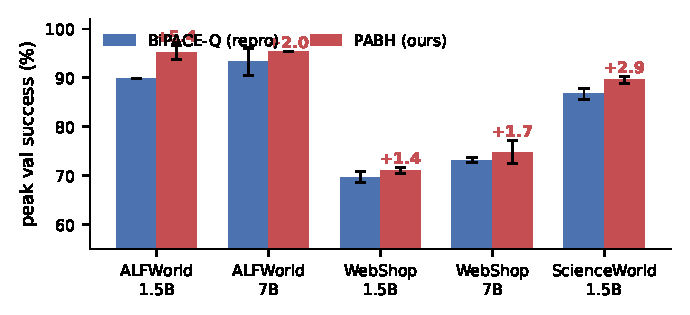
\includegraphics[width=\linewidth]{figs/fig_main_bars.pdf}
\caption{Peak validation success of BiPACE-Q (our same-pipeline
reproduction) vs.\ \method\ across environments and scales (error bars:
std over seeds).}
\label{fig:main_bars}
\end{figure}

\begin{figure}[t]
\centering
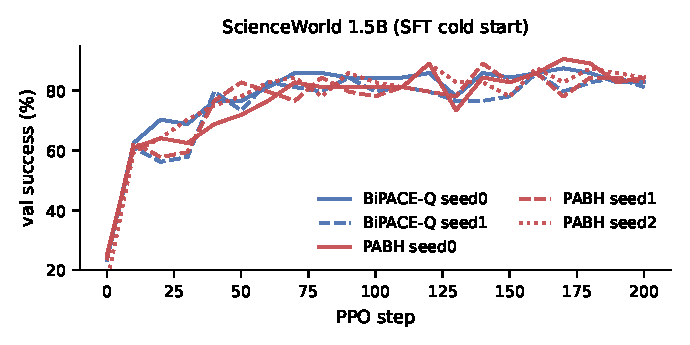
\includegraphics[width=\linewidth]{figs/fig_sw_curves.pdf}
\caption{Validation curves on ScienceWorld 1.5B (SFT cold start).
Every \method\ seed (red) dominates every BiPACE-Q seed (blue) in peak
success; shading-free for clarity (per-seed curves).}
\label{fig:sw_curves}
\end{figure}

\subsection{Anchor ablation: PRM vs.\ progress-set Jaccard}
\label{sec:anchor}

The PRM anchor beats the Jaccard anchor by \textbf{7.6\,pp} on ALFWorld
1.5B (95.2 vs.\ 87.5, single seed for Jaccard). We attribute
the gap to progress-set granularity: ALFWorld episodes complete
only 2--4 distinct subgoal events, so Jaccard distances are coarse and
nearly binary, while the four-level event PRM ($-0.1/0/0/0.5/1.0$)
preserves ordering information. \textbf{The anchor should preserve the
ordering structure of progress signals}; when progress sets are coarse
(few distinct subgoals per episode), a graded event PRM is the safer
default. Per-task breakdown (seed 0): the Jaccard variant wins on
\texttt{look\_at\_obj\_in\_light} (88.9 vs.\ 77.8) while PRM wins on
\texttt{pick\_two\_obj\_and\_place} (94.1 vs.\ 76.5)---anchors bias
\emph{which} task types receive the sharpest credit.

\subsection{Attribution: which layer carries the gain?}
\label{sec:attrib}

Our method is a three-layer stack; a natural question is whether the
gain comes from (i) progress-set text injection into the anchor
(state redefinition) or (ii) the trained metric (head). We run the
mid-arm: \gtext+actor\_hidden (state redefinition only, no head).
Table~\ref{tab:attrib} decomposes.

On 1.5B, the entire +5.3\,pp is carried by the \emph{trained metric}
(layer ii); text-level state injection alone is worthless ($-0.4$\,pp,
within noise). On 7B the layers split +1.2/+0.8\,pp. The
scale-dependence is mechanistic: 7B hidden-state clusters are already
dense and relatively pure (singleton 8--25\%, contamination half of
1.5B's, \S\ref{sec:e2}), so a trained metric has little pathology left
to fix; 1.5B's representation is weak, and metric learning pays most.
The layers are thus \emph{enabler}, not additive: \gtext\ carries no
independent gain on 1.5B, but it makes progress visible to the
embedding the head learns on---a result that informs how the stack
should be presented and tuned per scale.

\subsection{Purity, not coverage}
\label{sec:e2}

The GiGPO/BiPACE family reports singleton rate (fraction of ungrouped
steps) as the mechanism metric, defaulting to ``lower is better''. We
test this with a zero-GPU retrospective analysis: replay 16 completed
runs' logged trajectories, rebuild $\gset$ per step, cluster by
\emph{exact observation} (GiGPO's gold-standard grouping), and measure
(i) \textbf{conf\_clus}: fraction of multi-member clusters whose
members disagree in progress sets; (ii) \textbf{conf\_pair}: fraction
of intra-cluster pairs with different $\gset$; (iii) \textbf{var\_ratio}:
intra-cluster return variance over global variance; (iv) singleton rate.

\begin{figure}[t]
\centering
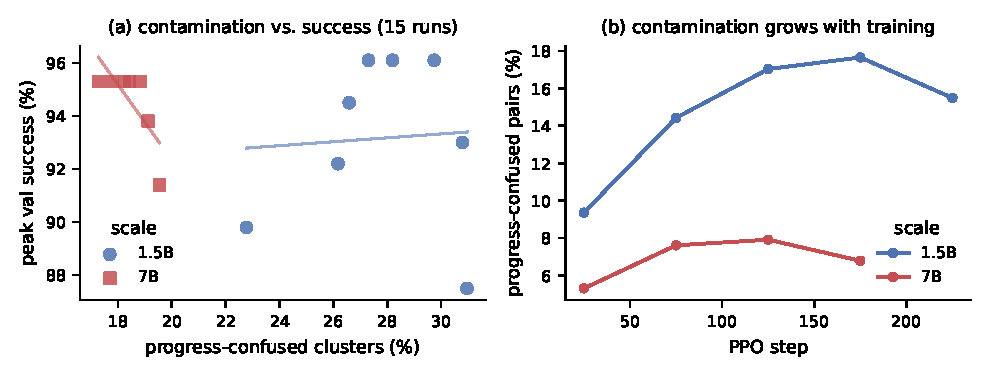
\includegraphics[width=\linewidth]{figs/fig_purity.pdf}
\caption{Retrospective purity analysis (16 runs, zero GPU).
(a) Progress-confused cluster fraction (exact-observation grouping)
vs.\ final success; each point is one run. (b) Contamination grows over
training in both scales---the pathology does not self-heal.}
\label{fig:purity}
\end{figure}

Three findings: (1) contamination \textbf{doubles over training}
(1.5B conf\_pair 8--11\% at s1-50 $\to$ 16--19\% at s151-200, all runs
consistent): as the policy specializes, same-start trajectories diverge
in progress paths, so same-observation/different-progress pairs
multiply---\emph{the pathology does not self-heal}. (2)
\textbf{Purity correlates with success}: conf\_clus vs.\ val
$r=-0.748$ at 7B ($-0.42$ at 1.5B), and the worst run is also the
dirtiest. (3) \textbf{Singleton is uninformative}: flat at 1.3--1.7\%
under exact matching with $r=+0.02$ vs.\ val; training-log singleton
(17--43\%) is likewise non-monotonic against success.
Coverage is a byproduct of metric quality, not a target---optimizing
singleton downward actively merges incomparable states and injects
biased advantages (BiPACE's own bound: group bias $\le2L\varepsilon$).

\subsection{SFT cold-start ablation (ScienceWorld)}
\label{sec:sft}

ScienceWorld's difficulty makes starting point a first-class variable.
With SFT cold-start, the 7B baseline starts at 46.9\% val and converges
to 89.1 peak/81.2 final; from raw Instruct weights it starts at 14.1\%
and is still climbing at the 150-step budget (67.2, $-14$\,pp below
SFT). The SFT row of the matrix (\S\ref{sec:main}) is thus the
meaningful comparison row for this environment; raw-start method arms
are in progress \todo{raw-start rows to be completed}.

\subsection{What did not work (ablation line)}
\label{sec:pabpo}

We document a systematic single-variable ablation line on ALFWorld 7B
against the full-method anchor (95.3): (i) MICo target rescale to fix
the head's output-range mismatch (upper bound 2 vs.\ target $\le3.0$)
\emph{collapses} the metric (clusters 305$\to$16)---scale and
$\varepsilon$ are coupled; a clamp variant is safe but yields no gain
(92.2/91.4); (ii) progress-conditioned action keys + local shrinkage
(D2b) reduces conf\_pair from 7--9\% to 2--4\% yet loses 1.9\,pp---a
static matching radius that over-merges spatially distinct states on
\texttt{Clean}-type tasks; (iii) a constant-trust variant recovers
\texttt{Clean} but loses on long-chain tasks (93.0--94.5); (iv) soft
kernel-weighted grouping (D1, $w_j=e^{-d/\sigma}$, $\sigma$ online
median-calibrated) and progress-conditioned policy input (PCAP) reach
89.1/93.8, not exceeding 95.3. Nine runs form a 92.2--94.5 band
\emph{below} the full method---evidence that the current stack's
components are jointly near a local optimum on ALFWorld 7B, and that
single-component action-side fixes do not transfer.

\subsection{The estimator ladder: GRPO $\to$ GiGPO $\to$ BiPACE-Q $\to$ \method}
\label{sec:gigpo_repro}

To isolate (a) the value of \emph{any} step-level credit and (b) the
value of a \emph{trained} step-level metric, we reproduce the full
estimator ladder on ALFWorld 1.5B under our pipeline: GRPO
(episode-level only), GiGPO (exact anchor grouping), BiPACE-Q
(approximate grouping), and \method\ (trained metric). The GiGPO point
doubles as the environment-gap calibration: it lands below its
published number by a margin comparable to BiPACE-Q's, as the
environment-gap account predicts.
\todo{ALFWorld GiGPO/GRPO reproduction in progress.}
On the new environment (ScienceWorld), where no published baseline
exists, we run the same ladder so that every comparison there is
contamination-free by construction
\todo{ScienceWorld GiGPO in progress; results added to
Table~\ref{tab:main}.}

%% ======================================================================
\section{Related Work}
\label{sec:related}

\paragraph{Group-based RL for LLM agents.} GRPO/RLOO established
within-group advantage estimation~\cite{grpo,rloo}; GiGPO extended it
to steps via anchor-state grouping~\cite{gigpo}; BiPACE made the
grouping approximate (BiGPO) and action-conditional
(PACE)~\cite{bipace}. Our work is a direct successor: it makes the
\emph{metric} underlying the approximate grouping trained and
progress-aware.

\paragraph{Bisimulation in deep RL.} DBC~\cite{dbc} learned
bisimulation metrics for control; MICo~\cite{micobisim} refined the
loss with target networks. We adapt MICo to the LLM-agent setting where
(i) rewards are terminal-sparse, necessitating progress-grounded
anchors, and (ii) the representation is a frozen LLM layer, so only a
projection head is trained.

\paragraph{Process rewards.} PRMs provide dense training signal in
reasoning~\cite{prm}; here the process signal shapes a \emph{state
metric} rather than the policy reward, keeping the PPO reward stream
unmodified (no reward-hacking surface).

%% ======================================================================
\section{Limitations}
\label{sec:limitations}

7B results use 1--2 seeds per arm; the Jaccard ablation on ALFWorld is
single-seed. The +1.6\,pp over official BiPACE-Q on ALFWorld 1.5B is
not statistically significant at $n{=}3$; our claim is \emph{parity
with a stronger-than-reproduced baseline}, with the +4.6--5.4\,pp
reproduction delta as the more meaningful effect size. Progress sets
require environment-specific parsers (closed template set in ALFWorld;
score deltas in ScienceWorld);
environments with open-ended feedback would need learned progress
detectors. ScienceWorld additional seeds and Sokoban validation are in
progress (\S\ref{sec:sft}).

%% ======================================================================
\section{Conclusion}
\label{sec:conclusion}

A 0.39M-parameter head, trained online with a progress-grounded MICo
loss on rollouts the PPO loop already produces, turns BiPACE's
syntactic state clustering into a learned value-equivalence metric at
no measurable cost---improving a strong baseline across four
interactive environments, with the clearest gains where the backbone's
representation is weakest (1.5B). The same machinery yields a
diagnostic: group purity, measurable offline, predicts run quality,
while the field's coverage metric does not. We hope the purity
perspective and the evaluation-protocol guidelines are as useful to the
community as the method itself.

%% ======================================================================
\bibliographystyle{ACM-Reference-Format}
\bibliography{refs}

\end{document}
